\documentclass[lang=en]{sjtuarticle}
\title{A Survey of PoS-like Consenses}
\author{Log Creative}
\sjtusetup{info/date={2024-04-10}}
\graphicspath{{figs/}}
\usepackage[style=ieee]{biblatex}
\addbibresource{ref.bib}
\usepackage[colorlinks]{hyperref}
\begin{document}
\maketitle
\section{PPC}
\subsection{Description}
Peercoin (PPC) \cite{ppc} is the first to introduce the Proof-of-Stake (PoS)
mechanism into the blockchain system in 2012. ``Stake'' here means the ``coin age'', i.e., currency amount $\times$ holding period.

In coin-stake transactions, each stakeholder is required to send coins to himself, which is used to generate a PPC block and obtain
partial revenue. The cost of gaining revenue is the consumption of coin age. The
PPC block requires participants to look for random
numbers (nonce) to make the hash value of the block header meet the
target difficulty. The target difficulty is inversely proportional to the coin
age consumed in coin-stake:
\begin{equation}
    H(H(B_\text{prev},A,t))\leq \mathit{balance}(A)m
\end{equation}
The more coin age accumulated by participants, the lower the bookkeeping difficulty,
and the greater the probability of generating blocks.

\subsection{Advantages}

\paragraph{It alleviates the energy and cost waste problem of PoW mining.} Compared with Bitcoins based on PoW (Proof-of-Work), the opportunity in PPC only
depends on the user's deposit in the system and the time of
saving the currency.

\paragraph{There is less motivation for the adversary to attack.} The cost of getting a large sum of coins in the
PoS system is higher than that of mastering most of the
computing power in the PoW system, since time is counted. Besides, once the block is generated, the coin age
will be immediately cleared (by the action of sending coins to himself), which also guarantees that an
attacker cannot continue the attack.

\subsection{Disadvantages}

\paragraph{Less active chain.} PoS encourages the behavior of hoarding. And since the coin age will also accumulate
when the node is offline, the node may prefer not to go
online.

\paragraph{Nothing-at-stake attack.} It is ``nearly'' costless to execute PoS protocol. With the aim of getting a reward,
nodes start supporting several branches of the chain. They can simply put their money in all chains without any fear of repercussion
at all. No matter what happens, they will always win and
have nothing to lose.

% \paragraph{Long-range attack.} 

\section{DPoS}

\subsection{Description}

DPoS (Delegated Proof of Stake) \cite{dpos} introduces two
roles called witness and delegate, both of which have
multiple members. DPoS mechanism is similar to the decision of the board
of directors in the real world. Stakeholders
with more than 51\% stakes can vote for the $N$ witnesses
and delegates. As shown in Figure \ref{fig:dpos}, the delegates are
responsible for voting and the witnesses just need to be
their follower nodes. The system calculates a certain number of delegates with the most votes based on the stakes of stakeholders, and the delegate takes turns to generate the block
in a prescribed order.

\begin{figure}[h]
    \centering
    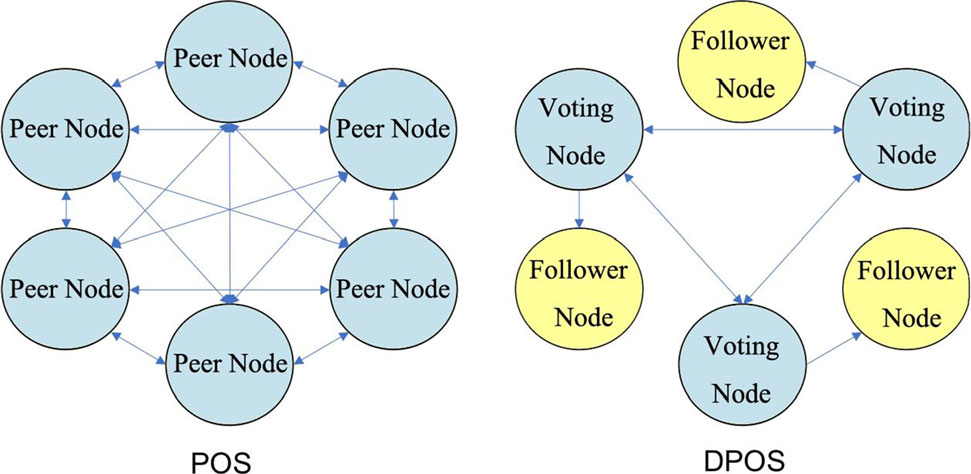
\includegraphics{DPoS.jpg}
    \caption{Node differences between PoS and DPoS}
    \label{fig:dpos}
\end{figure}

\subsection{Advantages}

\paragraph{Speed up the transaction.} The node does not have to wait
for confirmation of a considerable number of untrusted
nodes after the transaction is initiated, but only the delegate
needs to verify the transaction.

\paragraph{Make the chain active.} Since the block is signed by the delegates in turn, if a delegate is offline and misses signing the
block, he will face the risk of being replaced by other
candidate delegates. Therefore, the delegate must guarantee sufficient online time for the profit.

\subsection{Disadvantages}

\paragraph{Centralization.} With only a few delegates holding a considerable amount of power, this further makes DPoS vulnerable to vote buying.

\paragraph{Nothing-at-stack attack exists.} This verification is still not computationally intensive
and the parties can easily misbehave by voting for all blocks. This could be improved by another version of the DPoS protocol, where the node has to pay
a price to become a delegate, such as paying a deposit to a
security account \cite{bitshare2}.

%\section{Pure PoS}

%Pure Proof-of-Stake (Pure PoS) is a new consensus procedure implemented by the public blockchain
% called Algorand.

\section{FFG}

\subsection{Description}

The first version of Casper, the Friendly-Finality-Gadget (FFG) \cite{ffg} takes on the form of a hybrid PoW/PoS system based on BFT consensus theory. Casper FFG overlays an existing roof PoW blockchain, providing additional protections against block reversions.

In the simple version of Casper, there is a fixed set of validators and a proposal mechanism, which produces child blocks of existing blocks, forming an
ever-growing block tree. In the case of network
latency or deliberate attacks, the proposal mechanism will inevitably occasionally produce multiple children of
the same parent. Casper's job is to choose a single child from each parent. Casper only considers the subtree of checkpoints
forming the checkpoint tree, as shown in Figure \ref{fig:ffg}, where the dotted lines represent 99 blocks. A supermajority link colored in pink is an ordered pair of checkpoints such that at least $\frac{2}{3}$ of
validators (by deposit) have published votes.

\begin{figure}[h]
    \centering
    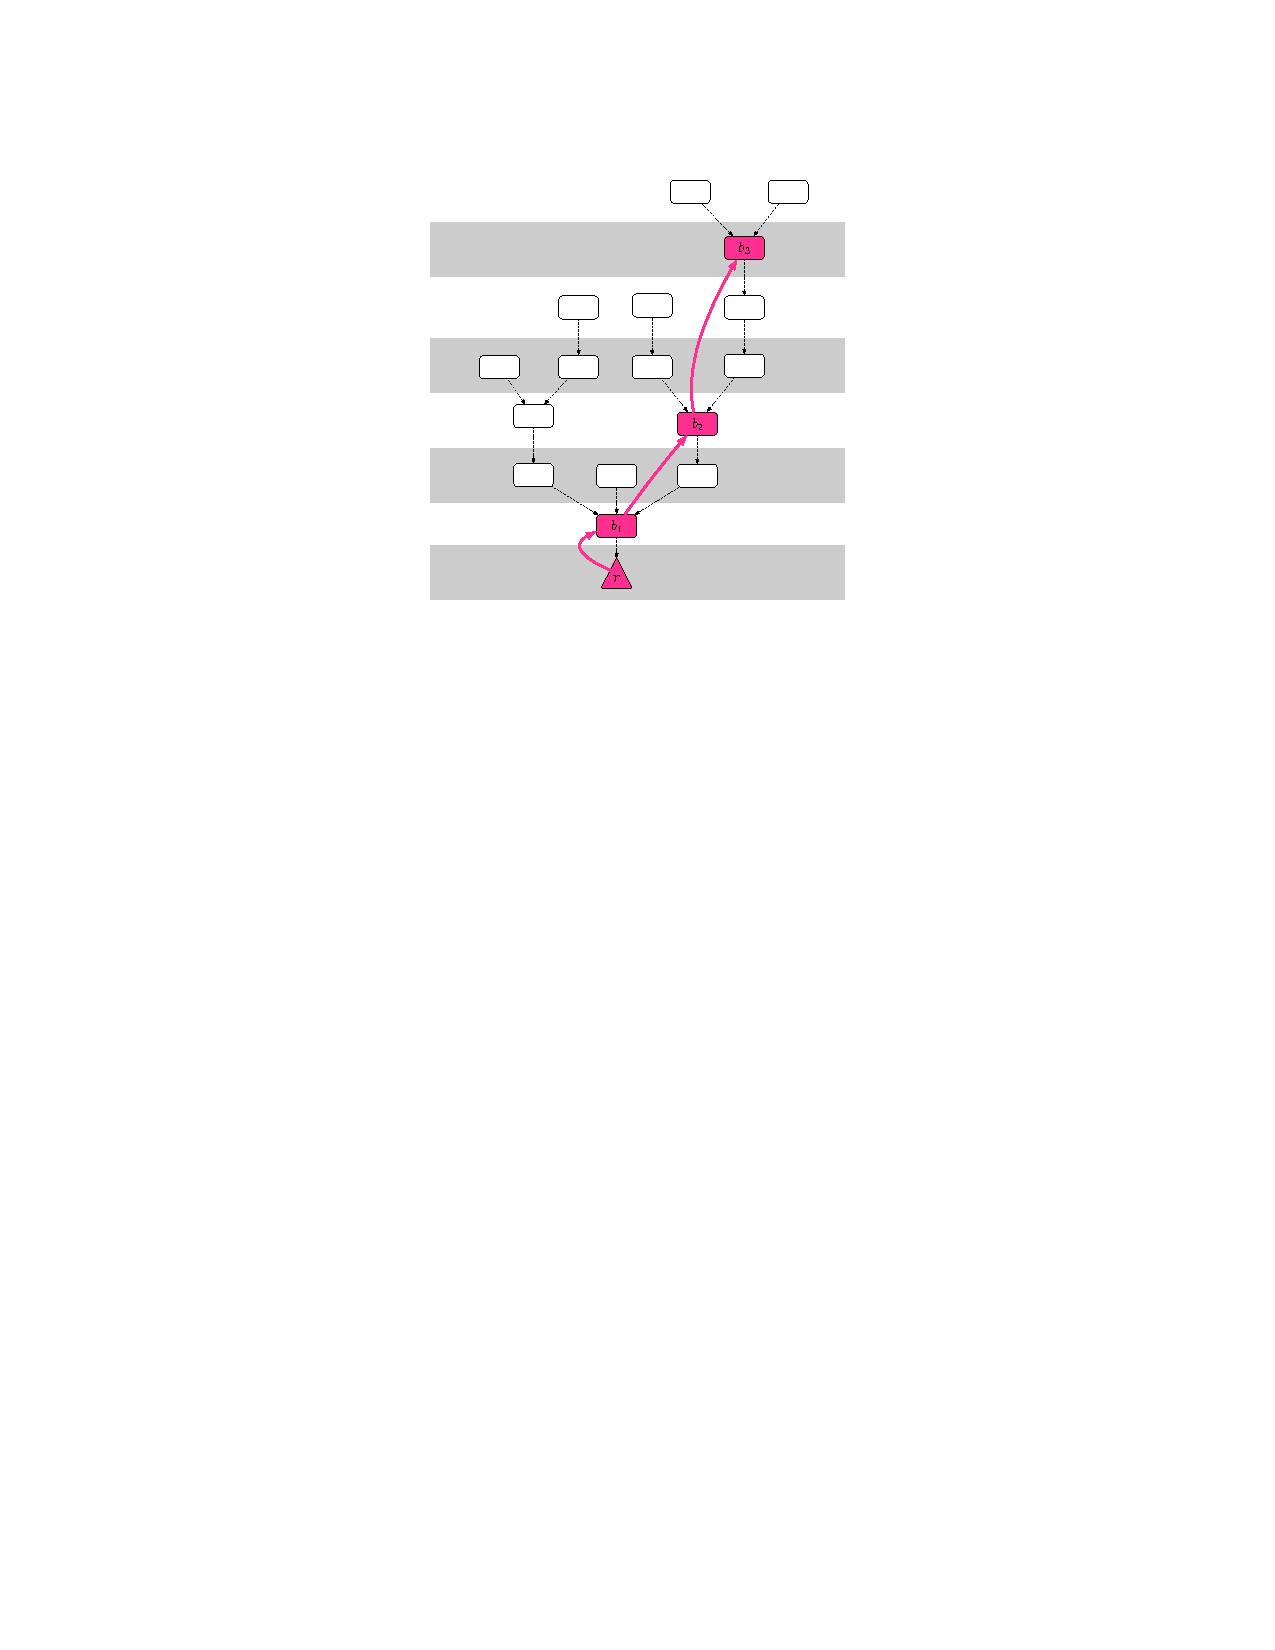
\includegraphics{FFG.pdf}
    \caption{Block tree with height and supermajority links in FFG}
    \label{fig:ffg}
\end{figure}

The most notable property of Casper is that it is impossible for any two conflicting checkpoints to be finalized
unless $\frac{1}{3}$ of the validators violate one of the two Casper Commandments/slashing conditions shown in Figure \ref{fig:ctwo}. If a validator violates the conditions, their entire deposit is forfeited, with a minor ``finder's fee'' provided to the individual who submitted the evidence transaction.

\begin{figure}[h]
    \centering
    \begin{tabular}[h]{|p{5cm}|p{5cm}|}
        \hline
        \multicolumn{2}{|p{10cm}|}{
            An individual validator $\nu$ must NOT publish two distinct votes
        }\\
        \hline
        $\langle\nu; s_1; t_1; \mathrm{h}(s_1); \mathrm{h}(t_1)\rangle$ & $\langle\nu; s_2; t_2; \mathrm{h}(s_2); \mathrm{h}(t_2)\rangle$ \\
        \hline
        \multicolumn{2}{|p{10cm}|}{
            such that either:\par
            I. $\mathrm{h}(t_1) = \mathrm{h}(t_2)$.
Equivalently, a validator must not publish two distinct votes for the same target height.\par
or\par
II. $\mathrm{h}(s_1) < \mathrm{h}(s_2) < \mathrm{h}(t_2) < \mathrm{h}(t_1)$.
Equivalently, a validator must not vote within the span of its other votes.
        } \\
        \hline
    \end{tabular}    
    \caption{The two Casper Commandments.}
    \label{fig:ctwo}
\end{figure}

FFG is more complicated than standard PoW designs. The fork choice rule is: Follow the chain containing the justified checkpoint of the greatest height. FFG also enables dynamic validator sets to prevent the attack of two conflicting checkpoints to both be finalized without any validator getting slashed.

FFG introduces several new features that BFT algorithms do not necessarily support: accountability, dynamic validators, defenses, and modular overlay.

\subsection{Advantages}

\paragraph{Plausible liveness.} This means that, no matter what has occurred in the past, if at least two-thirds of validators follow the protocol, it's always possible to finalize a new checkpoint without any validator violating a slashing condition.

\paragraph{Robust to attacks.} For ``nothing-at-stake'' attacks, FFG introduces the betting mechanism. For long-range attacks, the node must regularly update the latest blocks and forbid revert blocks that have been finalized. For catastrophic crashes, Casper FFG introduces the “Inactivity Leak.”

\subsection{Disadvantages}

\paragraph{51\% attack.} A wholly compromised block proposal mechanism will prevent Casper
from finalizing new blocks. The problem that Casper does not wholly solve, particularly related to 51\% attacks, can still be corrected using
user-activated soft forks.

\paragraph{Parallel voting.} This contract version of Casper FFG was later deprecated. \cite{deprecate} In the contract version, it is assumed that the votes can be processed in parallel, but there are many intermediate states in calculating the voting reward. The order of voting processing will affect the final state, which means that the parallelization will make the consensus unreachable. This is fixed by Ethereum 2.0, which integrates Casper FFG with other optimization proposals (such as sharding) \cite{eth2}.

\printbibliography
\end{document}